\section{DNS theory}

\subsection{The data contained in name servers}


Name servers manage two kinds of data:

\begin{enumerate}
\item The first kind of data held in sets called \Cola{zones}; each zone is the
  complete database for a particular ``pruned'' subtree of the domain space.
  This data is called \Cola{authoritative}. \colz{A name server periodically
    checks to make sure that its zones are up to date, and if not, obtains a new
    copy of updated zones from \cola{master files stored locally} or in
    \cola{another name server}.
  }
\item The second kind of data is \cola{cached data} which was acquired by a
  local resolver.
\end{enumerate}

Depending on its capabilities, a name server could be a standalone program on a
dedicated machine or a process or processes on a large timeshared host. A simple
configuration might be shown in \cref{fig:name-serv-arch}

\begin{figure}[h]
  \centering
  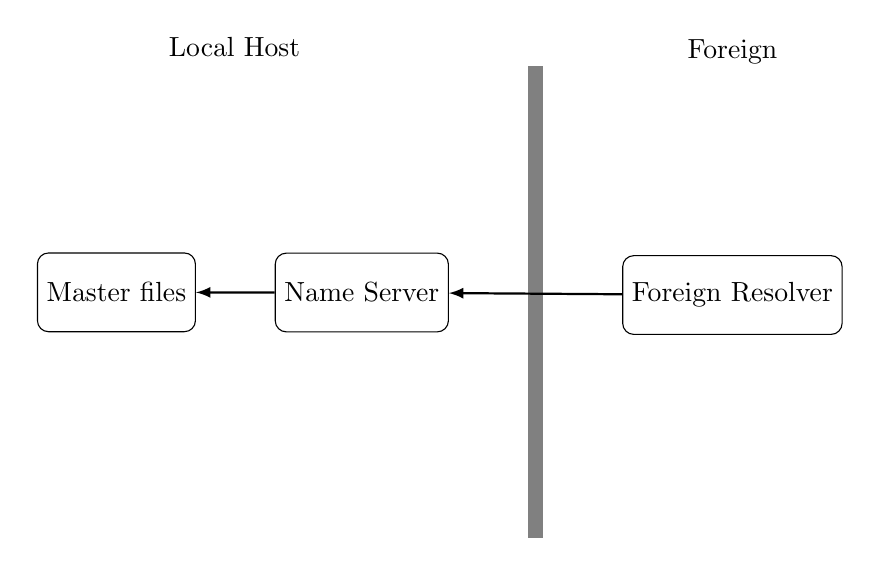
\begin{tikzpicture}
    % \draw[step=1cm,help lines,] (-7.5cm,-5cm) grid +(15cm,10cm);
    \tikzstyle{every node}=[draw=black,anchor=base]
    \matrix[draw=none,column sep=1cm,nodes={minimum size=1cm, rounded corners}] {
      \node[name=mf] {Master files}; &
      \node[name=ns] {Name Server}; &

      \newdimen\x
      \newdimen\y
      \x=3cm
      \y=0.1cm
      \fill[gray] (-\y,-\x) rectangle +(2\y,2\x); &
      \node[name=fr] {Foreign Resolver};\\
    };

    \node[draw=none] at ([shift={(1.5cm,3cm)}]mf) {Local Host};
    \node[draw=none] at ([shift={(0,3cm)}]fr) {Foreign};

    \draw[latex-,thick] (mf) -- (ns);
    \draw[latex-,thick] (ns) -- (fr);
  \end{tikzpicture} 
  \caption{Simple name server architecture}
  \label{fig:name-serv-arch}
\end{figure}

% \clearpage{}

\subsection{The Resource Record (RR) definitions}
\label{sec:rr-defs}

\subsubsection{Format}

All Resource Record (RR) have the same top level format shown in
\cref{tab:rr-format}. The numbers are all big-endien. (the ``internet-endien'')

\newcolumntype{s}{>{\hsize=.2\hsize}X}
\newcolumntype{c}{>{\hsize=.2\hsize \centering\arraybackslash}X}
\begin{table}[h]
  \centering
  \begin{tabularx}{0.8\linewidth}{scX}
    Field& Length (word = 2 bytes) & Description \\[2pt]
    \hline
    \texttt{Name} & 4 & The name of owner, i.e. the node to which this RR pertains. \\[1pt]
    \texttt{Type} & 1 & The RR \texttt{TYPE} code. \\[1pt]
    \texttt{Class} & 1 & The RR \texttt{CLASS} code.\\[1pt]
    \texttt{TLL} & 2 & \texttt{int32} that specifies the time interval that the
                       resource record may be cached before the source of the
                       information should again be consulted. \colz{Zero
                       values are interpreted to mean that the RR can only be
                       used for the transaction in progress, and should not be
                       cached. For example,  \cola{SOA records} are always distributed
                       with a zero TTL to prohibit caching. Zero values can also
                       be used for very volatile data.
                       } \\[1pt]
   \texttt{RDLENGTH} & 2 & \texttt{uint16} that specifies the length in octets
                           of \texttt{RDATA} field. \\[1pt]
         \texttt{RDATA} & variable & The string that describes the resource.
  \end{tabularx}
  \caption{RR top level format}
  \label{tab:rr-format}
\end{table}

\FloatBarrier                   % \usepackage{placeins}

\subsubsection{\texttt{TYPE} values}
Following \texttt{TYPE} fields are available (\cref{tab:rr-types}):
\label{sec:rr-types}
\begin{table}[h]
  \centering
  \begin{tabularx}{0.8\linewidth}{scX}
    TYPE& value & meaning \\[2pt]
    \hline
    \texttt{A} & 1 & a host address \\
    \texttt{NS} & 2 & an authoritative name server \\
    \texttt{CNAME} & 5 & the canonical name for an alias \\
    \texttt{SOA} & 6 & marks the start of a zone of authority \\
    \texttt{WKS} & 11 & a well known service description \\
    \texttt{PTR} & 12 & a domain name pointer \\
    \texttt{HINFO} & 13 & host information \\
    \texttt{MINFO} & 14 & mailbox or mail list information \\
    \texttt{MX} & 15 & mail exchange \\
    \texttt{TXT} & 16 & text strings \\
  \end{tabularx}
  \caption{Defined \texttt{TYPE} values}
  \label{tab:rr-types}
\end{table}

\cSay{
  \colz{
    You may have noticed that some of the values are missing, e.g. \texttt{3,
      4}. Those are either obsolete or experimental.
  }
}

\texttt{TYPE} values are in fact subset of \texttt{QTYPE} values. \texttt{QTYPE}
values that are not \texttt{TYPE} values are shown in \cref{tab:qtypes}.

\begin{table}[h]
  \centering
  \begin{tabularx}{0.8\linewidth}{scX}
    QTYPE& value & meaning \\[2pt]
    \hline
    \texttt{AXFR} & 252 & A request for a transfer of an entire zone \\
    \texttt{MAILB} & 253 & A request for mailbox-related records \\
    \texttt{*} & 255 & A request for all records \\
  \end{tabularx}
  \caption{Defined \texttt{QTYPE} values}
  \label{tab:qtypes}
\end{table}

\subsubsection{\texttt{CLASS} values}

You just need to remember one value: \texttt{IN} (value=1) which stands for
``internet''.

\subsubsection{\texttt{CNAME RDATA} format}

\texttt{CNAME} RDATA just contains a \cola{domain name}, which is represented as
a series of labels, and terminated by a label with zero length. 

\subsection{Message}

All DNS messages have the same top level format shown in \cref{tab:msg-format}.

\begin{table}[h]
  \centering
  \begin{tabularx}{0.8\linewidth}{sX}
    Field & Description \\[2pt]
    \hline
    \texttt{Header} & A fixed format header. \\
    \texttt{Question} & the question for the name server. \\
    \texttt{Answer} & RRs answering the question. \\
    \texttt{Authority} & RRs pointing toward an authority. \\
    \texttt{Additional} & RRs holding additional information. \\
  \end{tabularx}
  \caption{The DNS message format}
  \label{tab:msg-format}
\end{table}

\subsubsection{Header}

The header contains the following fields (\cref{tab:msg-header}).


\begin{table}[h]
  \centering
  \begin{tabularx}{0.8\linewidth}{scX}
    field & size (bits) & meaning \\[2pt]
    \hline
    \texttt{ID} & 16 & Id assigned by the \cola{program that
                       generates the query}. \colz{
                        This id is copied the corresponding reply and
                       can be used by the \colZ{requester} to match up replies
                       to outstanding queries.
                       } \\
    \texttt{QR} & 1 & \colz{
                      A one bit field that specifies whether this message is a
                      \colZ{query (0), or a response (1).}} \\
    \texttt{OPCODE} & 4 & \colz{
                          the kind of query. It can be
                          \begin{align*}
                            0 &\quad \Rightarrow \text{a standard query (QUERY)}\\
                            1 &\quad \Rightarrow \text{an inverse query (IQUERY)}\\
                            2 &\quad \Rightarrow \text{a server status
                                request}\\
                            3-15 &\quad \Rightarrow \text{reserved for future use}
                          \end{align*}
                          }
  \end{tabularx}
  \caption{The DNS message header format}
  \label{tab:msg-header}
\end{table}